\subsection{MCQ Generator}
In this part, we will fine-tune the \textbf{google/flan-t5-base} model to generate multiple-choice questions from text. The initial "zero-shot" performance of the base model was poor, producing malformed and repetitive outputs. To solve this, we employed a Parameter-Efficient Fine-Tuning (PEFT) method called LoRA.
\subsubsection{Zero-Shot Testing}
We began by testing the model's "zero-shot" capability. We provided a prompt containing a context passage and the instruction, "Generate one multiple-choice question..."\\
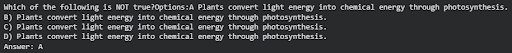
\includegraphics[scale = 0.9]{experiements/image/zero.png}

\subsubsection{Dataset Selection \& Fine-Tuning Process}
RACE (Reading Comprehension from Examinations): This dataset was selected as the ideal solution. Loaded from the Hugging Face Hub (race, high subset), it provided the four essential components: article, question, options, answer.\\
1 Epoch on Full Data (approx. 62,000 training examples, 3,400 validation examples):\\
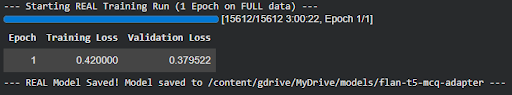
\includegraphics[scale = 0.9]{experiements/image/epoch.png}\\
The model produced distinct options for A, B, C, and D, but it generated the wrong answer. It had successfully learned the format (syntax) of an MCQ but had not yet learned the reasoning (semantics) to consistently identify the correct answer.